%%% Local Variables:
%%% mode: latex
%%% TeX-master: "../doc"
%%% coding: utf-8
%%% End:
% !TEX TS-program = pdflatexmk
% !TEX encoding = UTF-8 Unicode
% !TEX root = ../doc.tex

This section shows the results achieved during realization of the project.

\section{Application data persistence with LocalStorage}
To store application data (plan project data, data fetched from Toggl etc.), the approach described in chapter \ref{Local Storage} was applied. The data is hold by a data manager object which is stored in Local Storage and can be loaded from there using the interface provided by the LocalStorage library.

\section{Overview PlanProject vs TogglProject} \label{Graphical overview}
To display the difference between the plan projects and the corresponding Toggl project, three different charts are displayed in the charts tab.
\begin{itemize}
	\item Total overview
	\item Projects overview
	\item Project time range overview
\end{itemize}
The different charts are explained in more detail in the following subsections.

\subsection{Total Overview}
This bar chart shows the overall sum of the time planned for all plan projects, compared to the total tracked time of their associated Toggl projects. Additionally, a prediction of how much time will be needed according to the future plan entries is displayed. An example for two projects is shown in \ref{figure9}.
\begin{figure}[H]
	\centering
	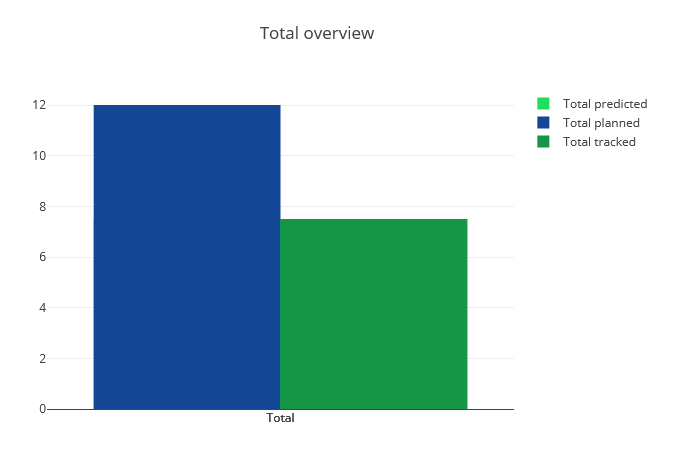
\includegraphics[width=1.0\columnwidth]{TotalOverview}
	\caption{Total overview for two projects}
	\label{figure9}
\end{figure}
If all projects have been completed already, meaning there are no future plan entries for any project, then no prediction will be displayed. An example for one project is shown in \ref{figure10}.
\begin{figure}[H]
	\centering
	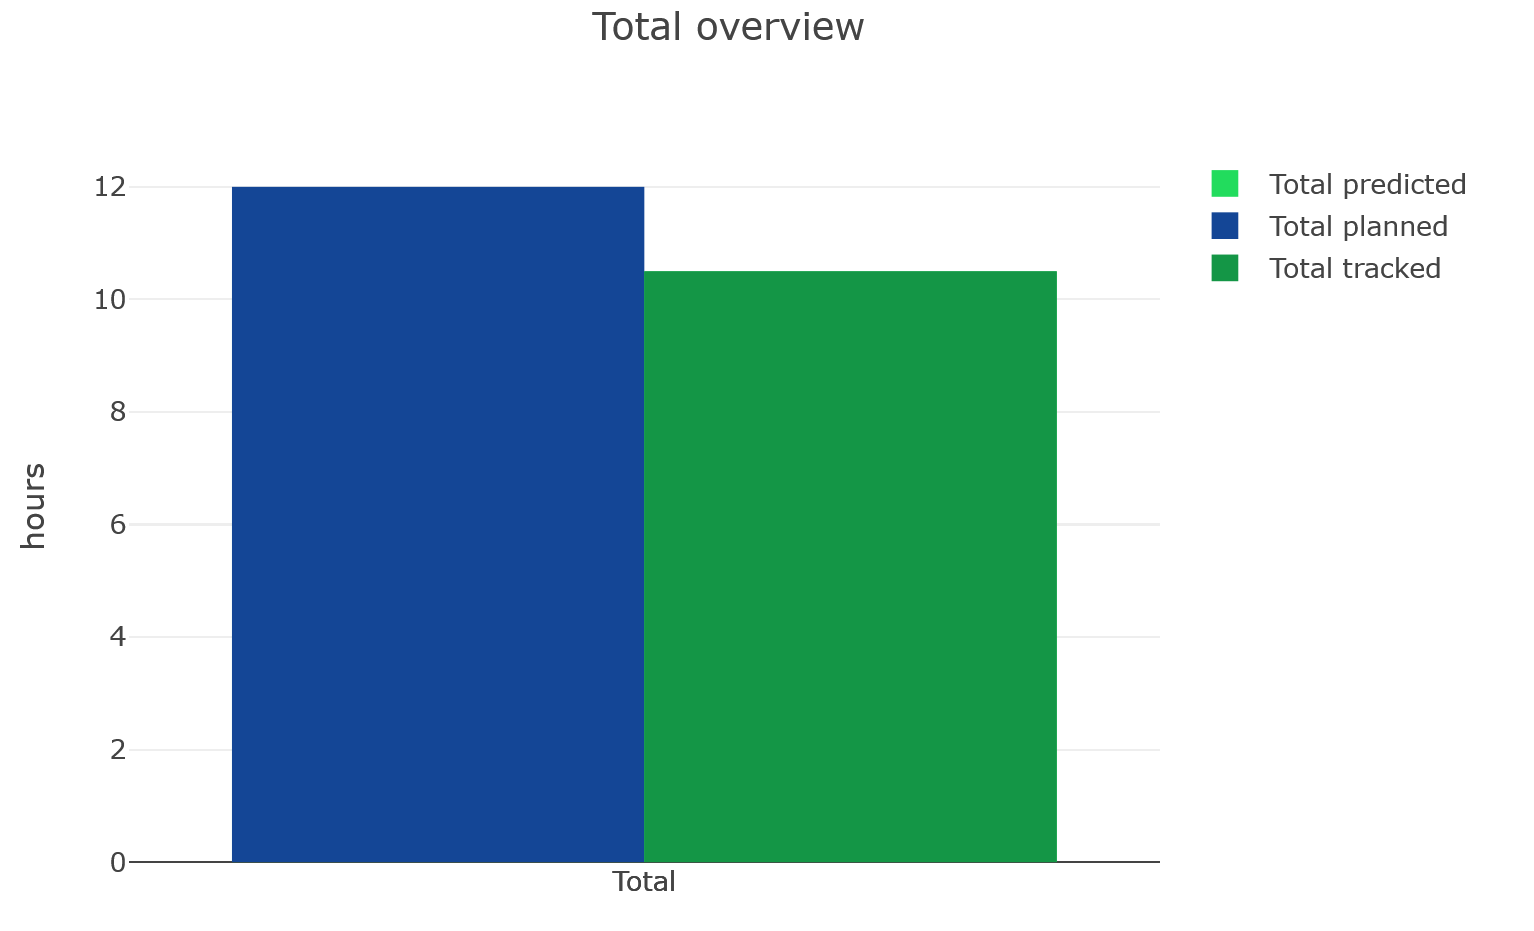
\includegraphics[width=1.0\columnwidth]{TotalOverview_FinishedProject}
	\caption{Total overview for one finished project}
	\label{figure10}
\end{figure}

\subsection{Projects Overview}
This bar chart is similar to the total overview, but the single projects are displayed separately. An other minor difference is that the prognosis is added to both the tracked time and the planned time, creating a prediction for both. An example for two projects is shown in \ref{figure10}.
\begin{figure}[H]
	\centering
	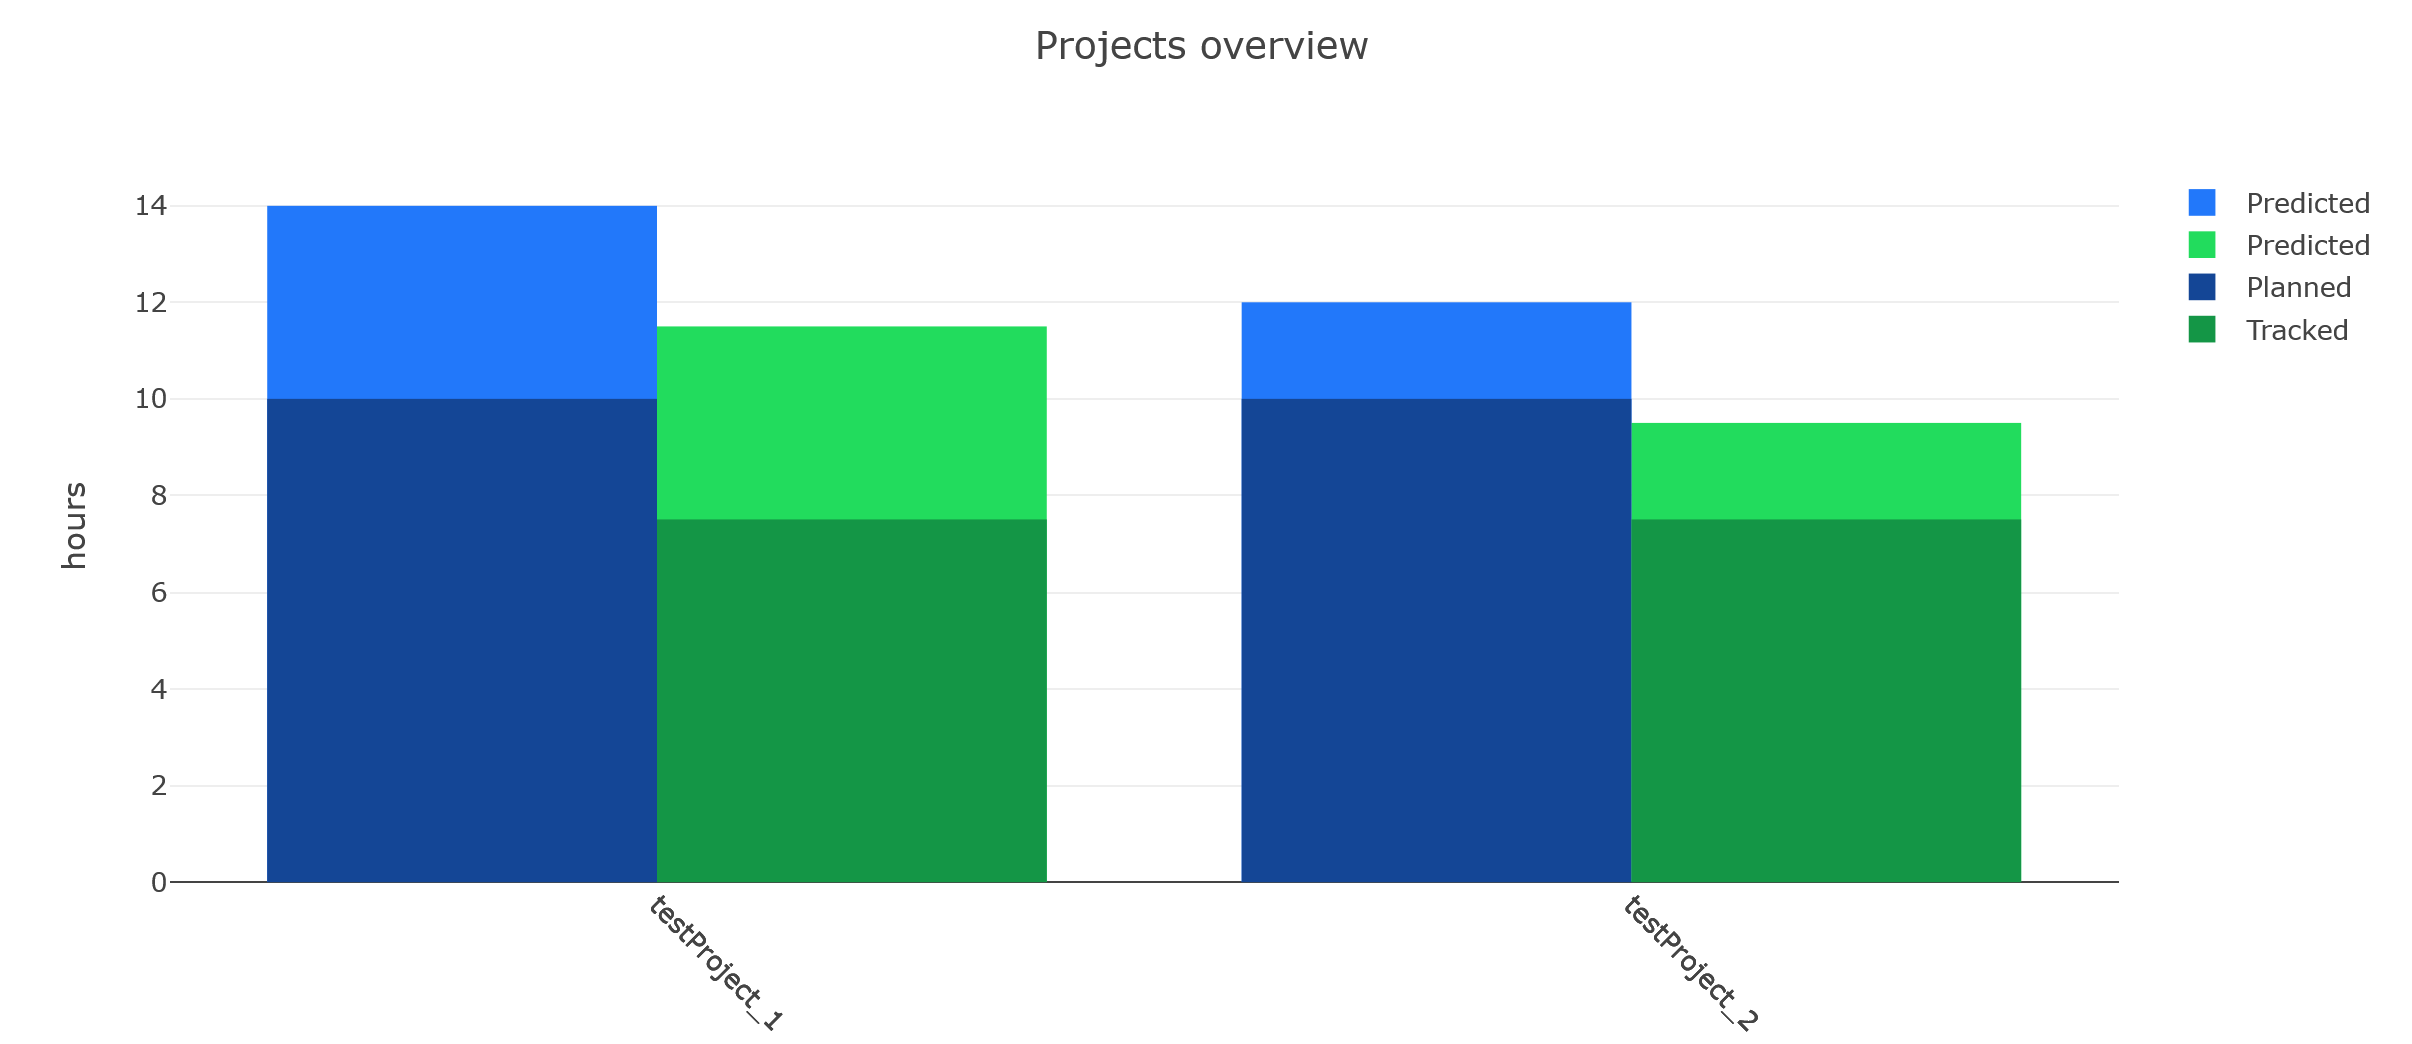
\includegraphics[width=1.0\columnwidth]{ProjectOverview}
	\caption{Project overview for two projects}
	\label{figure11}
\end{figure}
If a project has been completed already, meaning there are no future plan entries for it, then no prediction will be displayed for that project. An example for one project is shown in \ref{figure12}.
\begin{figure}[H]
	\centering
	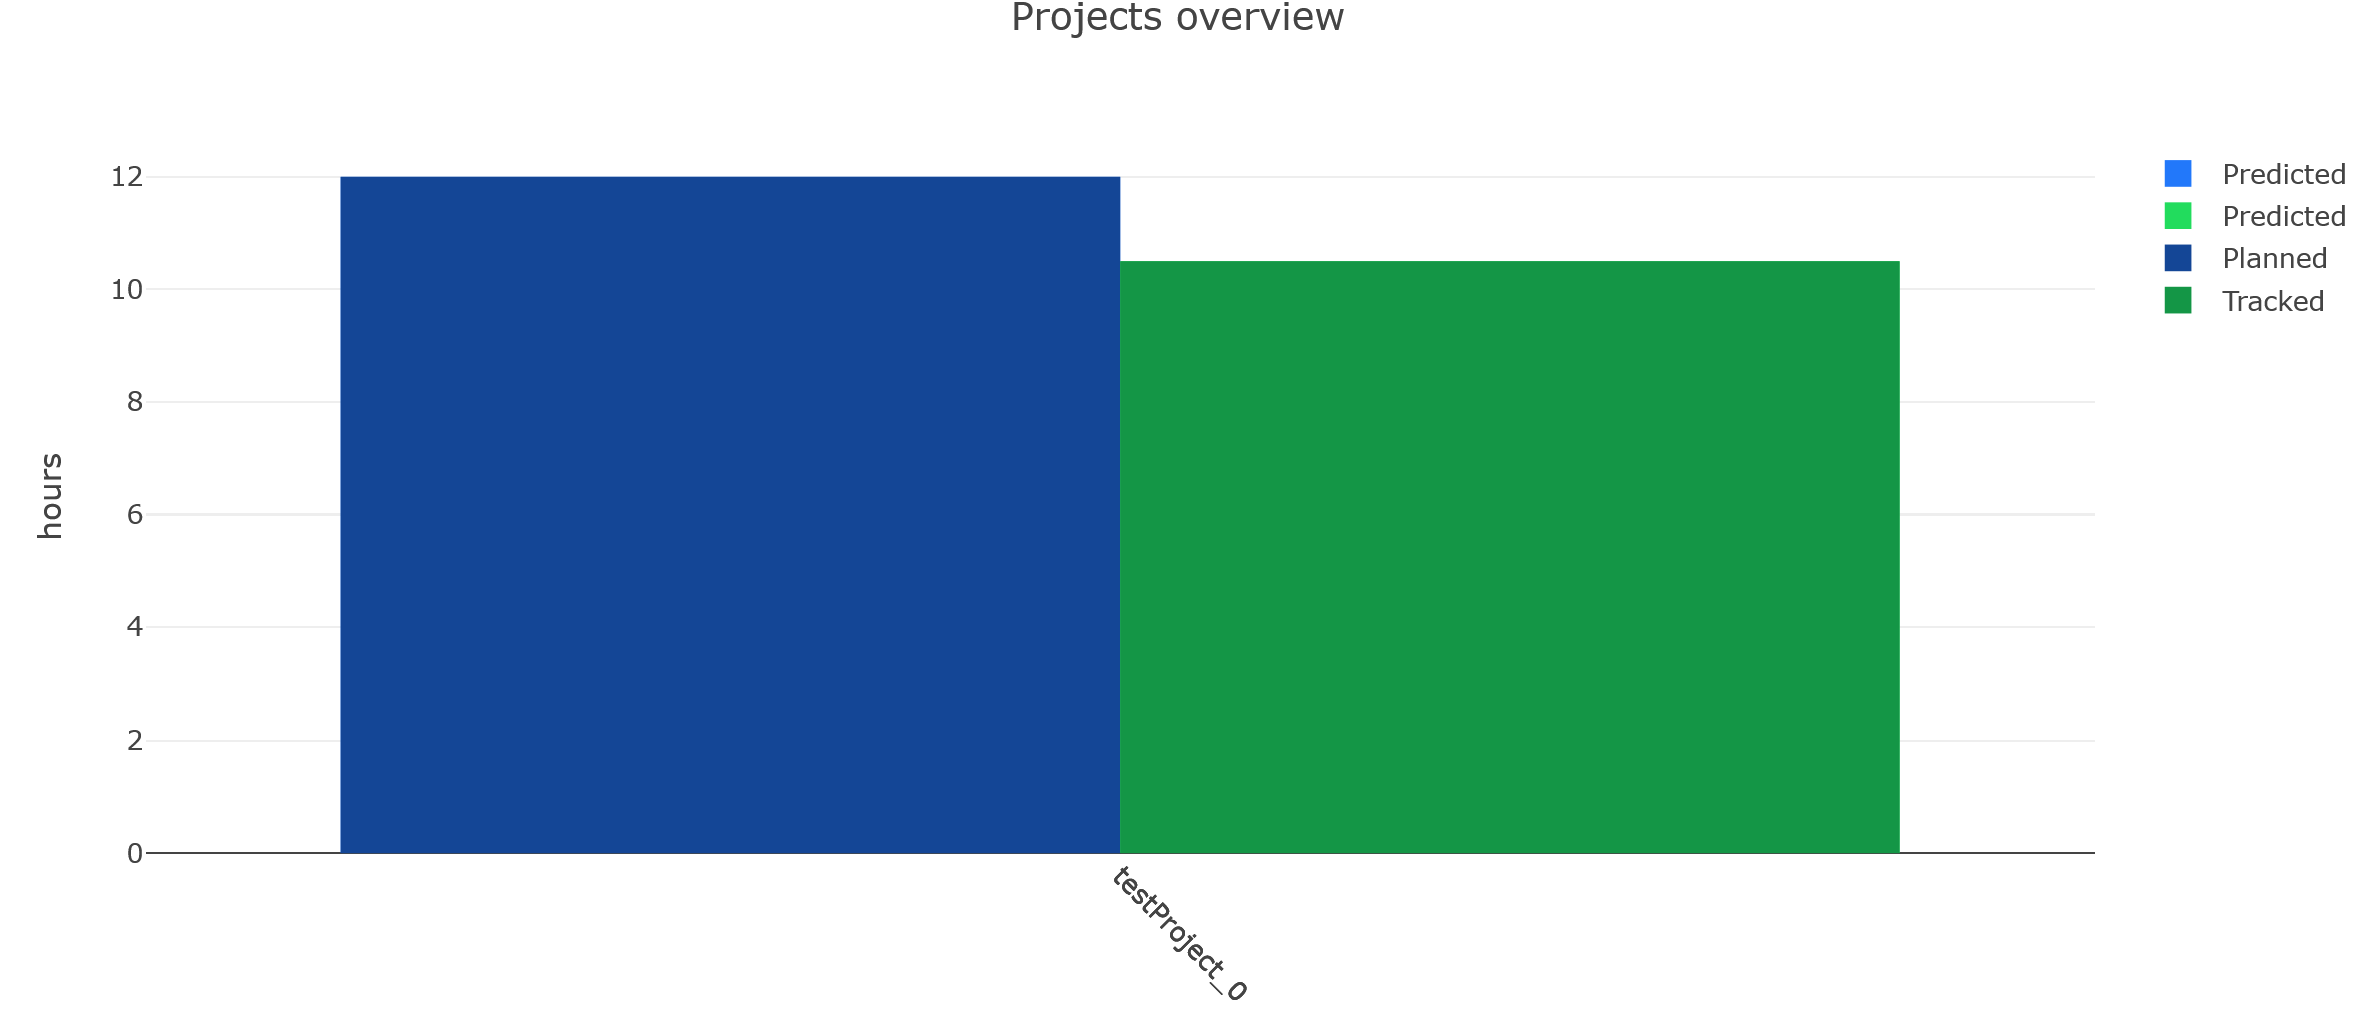
\includegraphics[width=1.0\columnwidth]{ProjectOverview_FinishedProject}
	\caption{Project overview for one finished project}
	\label{figure12}
\end{figure}

\subsection{Project time range overview}
To display the chart, the user first has to choose the applicable time range. On hitting the "Set filter" button, the time range is set, and a line chart is drawn for every project, showing the development of planned time and tracked time during the selected time range. To reset the filter, the "Reset filter" button has to be hit. This chart allows to see how the time amounts displayed in the other charts have been achieved and thus allows a user to estimate the quality of their planning. An example for one project is shown in \ref{figure11}.
\begin{figure}[H]
	\centering
	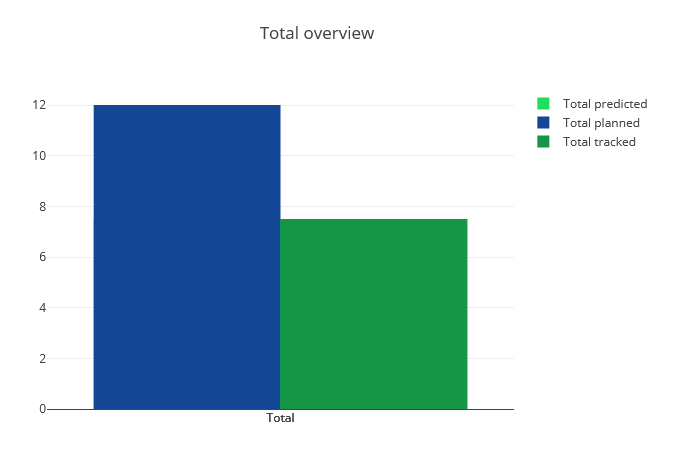
\includegraphics[width=1.0\columnwidth]{TimeOverview}
	\caption{Time overview for one project}
	\label{figure13}
\end{figure}

\section{Application status display and synchronization} \label{Status display}
In the original prototype, a Blazor page for synchronization with Toggl had already been added. As described in chapter \ref{JS replacement}, the modal entry mask was replaced by blazor input components (see picture \ref{Toggl page initial}). When the "Save Toggl settings" button is clicked, the credentials entered in the text fields are saved using Local Storage (see chapter \ref{Local Storage}), and a first synchronization request is sent to Toggl. If one or both fields are left empty, appropriate error messages are displayed (see picture \ref{Toggl page validation}). After successful synchronization, the entry fields and the save button are replacaed by a "Synchronize" button in order to allow users to re-synchronize the ATP with Toggl at any time and not just on entering the Toggl credentials. A label next to the button indicates the time of the last synchronization. Below the button, an overview of the loaded data and their associations with the ATP planning data is displayed, see picture \ref{Toggl associated}. If a Toggl project has no associations yet, this is indicated in the load overview (see picture \ref{Toggl loaded}). Entries which do not belong to a Toggl project are displayed as belonging to "Entries without project" (see picture \ref{Toggl no project}). Internally, these entries are saved in a project having this name. Toggl projects which have been deleted in Toggl, but are still present in the ATP, are marked as deleted (see picture \ref{Toggl deleted}). They will be present in the ATP until Local Storage is cleared (e. g., when the browser cache is cleared).

\begin{figure}[H]
	\centering
	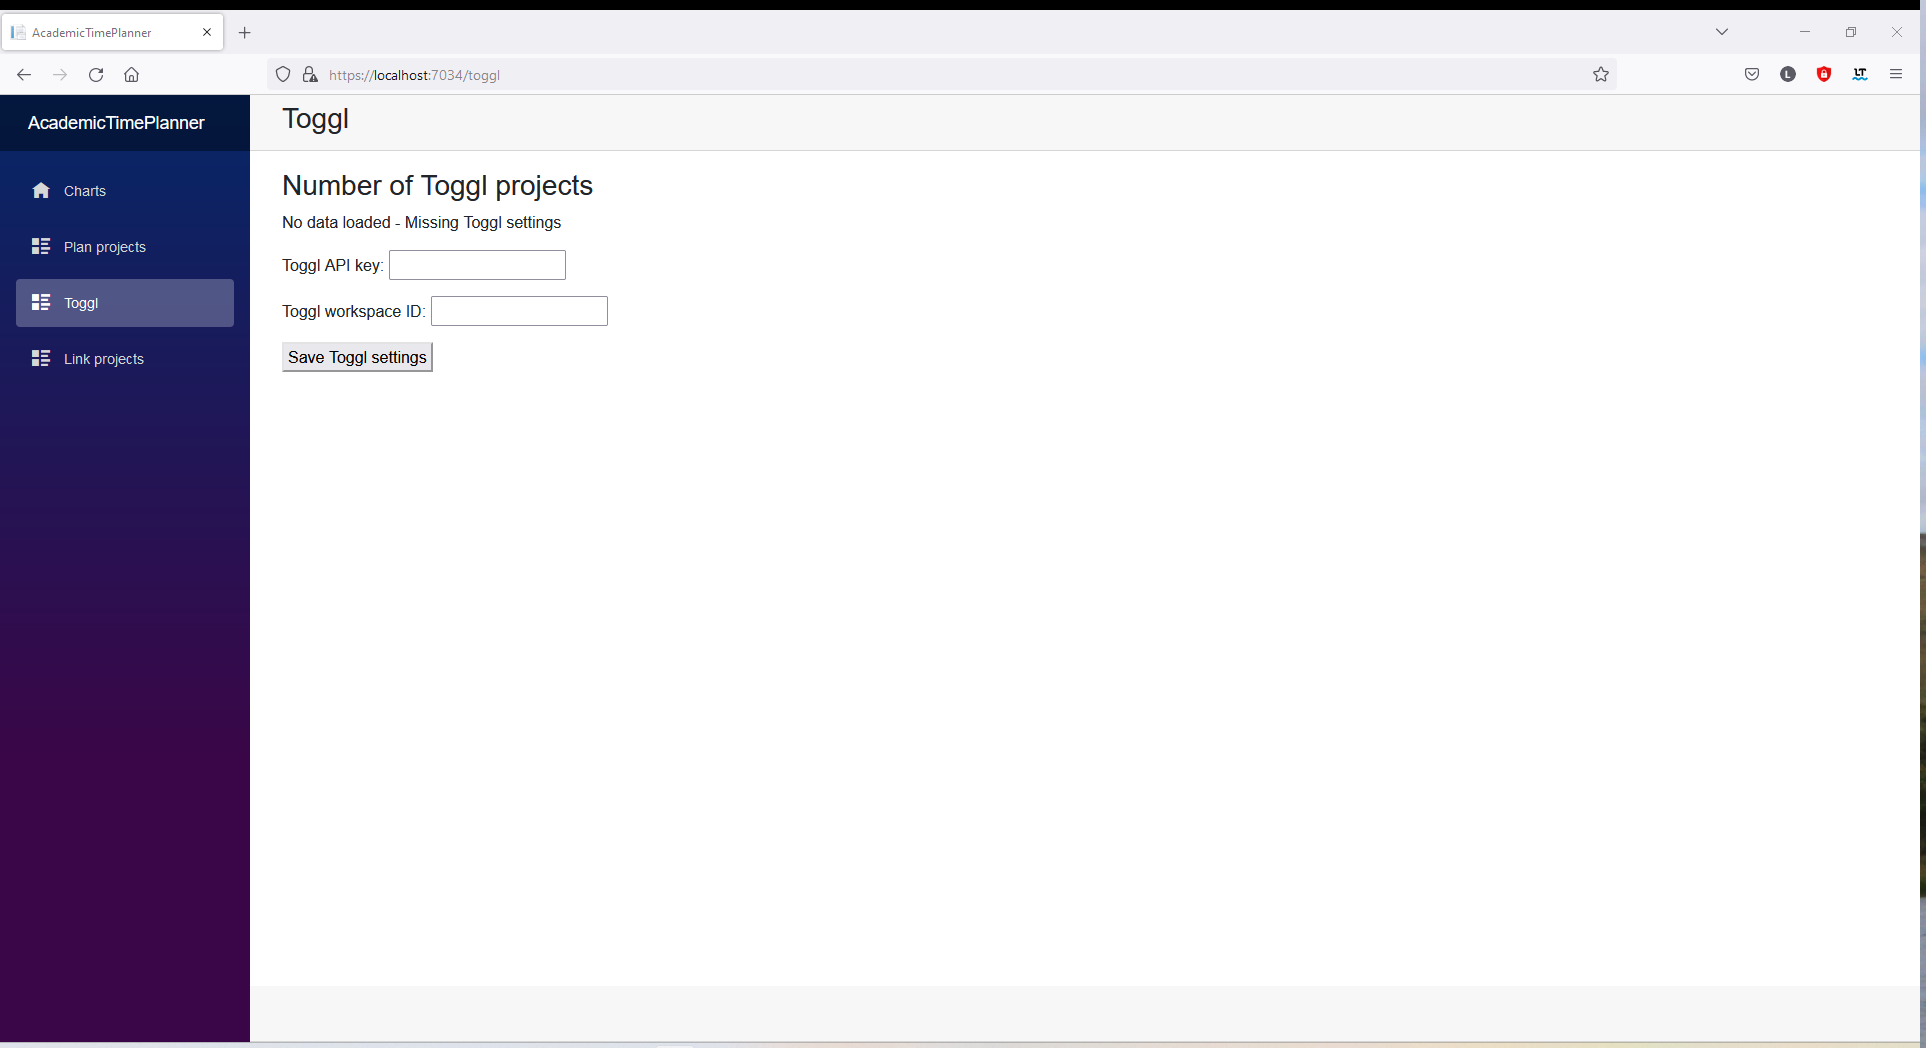
\includegraphics[scale=0.75]{Toggl_init}
	\caption{Toggl page with no Toggl projects loaded and no synchronization done yet}
	\label{Toggl page initial}
\end{figure}

\begin{figure}[H]
	\centering
	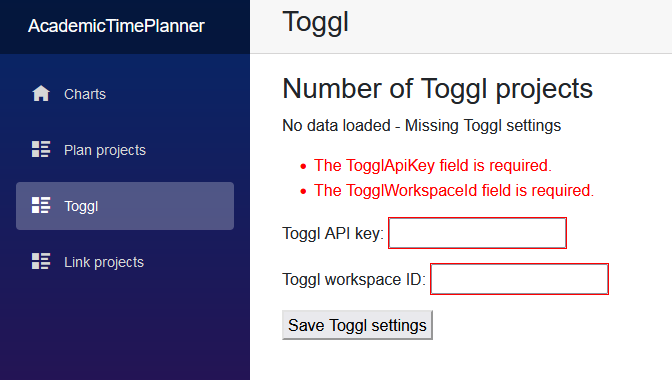
\includegraphics[scale=0.75]{Toggl_validation}
	\caption{Toggl page with empty credentials input}
	\label{Toggl page validation}
\end{figure}

\begin{figure}[H]
	\centering
	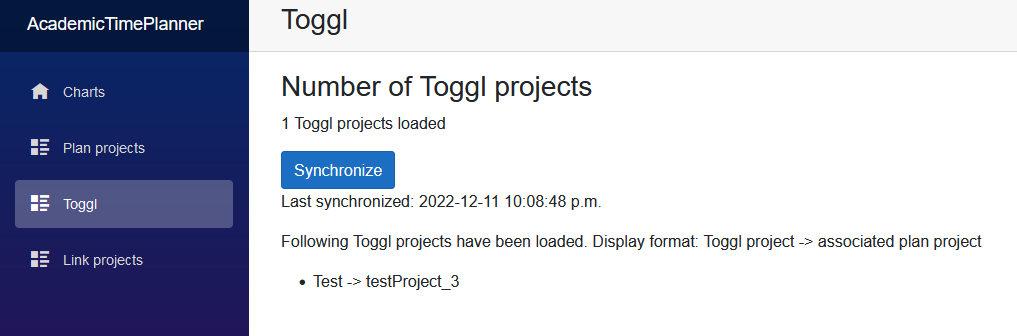
\includegraphics[scale=0.75]{Toggl_associated}
	\caption{Toggl page after loading of one Toggl project which is associated to a plan project}
	\label{Toggl associated}
\end{figure}

\begin{figure}[H]
	\centering
	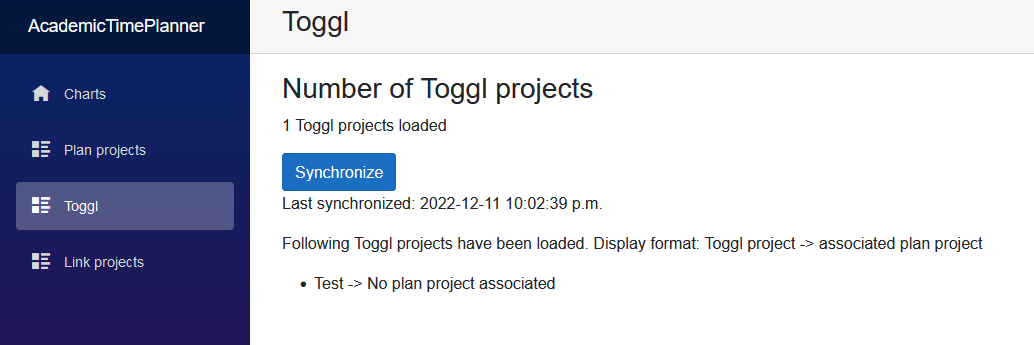
\includegraphics[scale=0.75]{Toggl_loaded}
	\caption{Toggl page after loading of one Toggl project which is not associated to any plan project}
	\label{Toggl loaded}
\end{figure}

\begin{figure}[H]
	\centering
	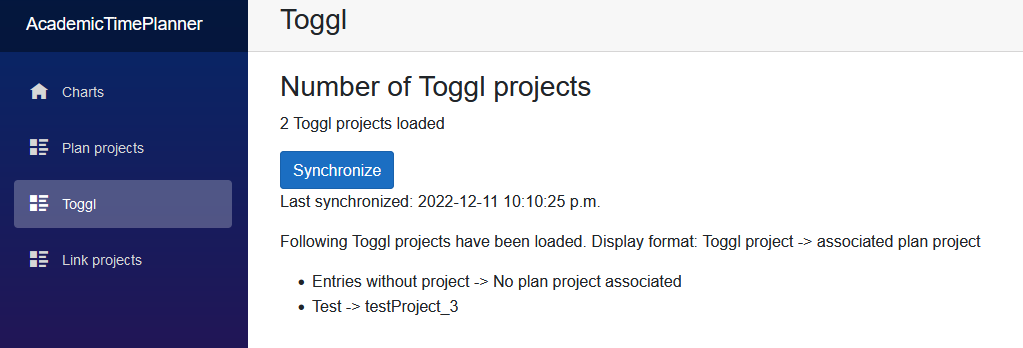
\includegraphics[scale=0.75]{Toggl_noProject}
	\caption{Toggl page after loading of a Toggl project and some entries which do not belong to a Toggl project}
	\label{Toggl no project}
\end{figure}

\begin{figure}[H]
	\centering
	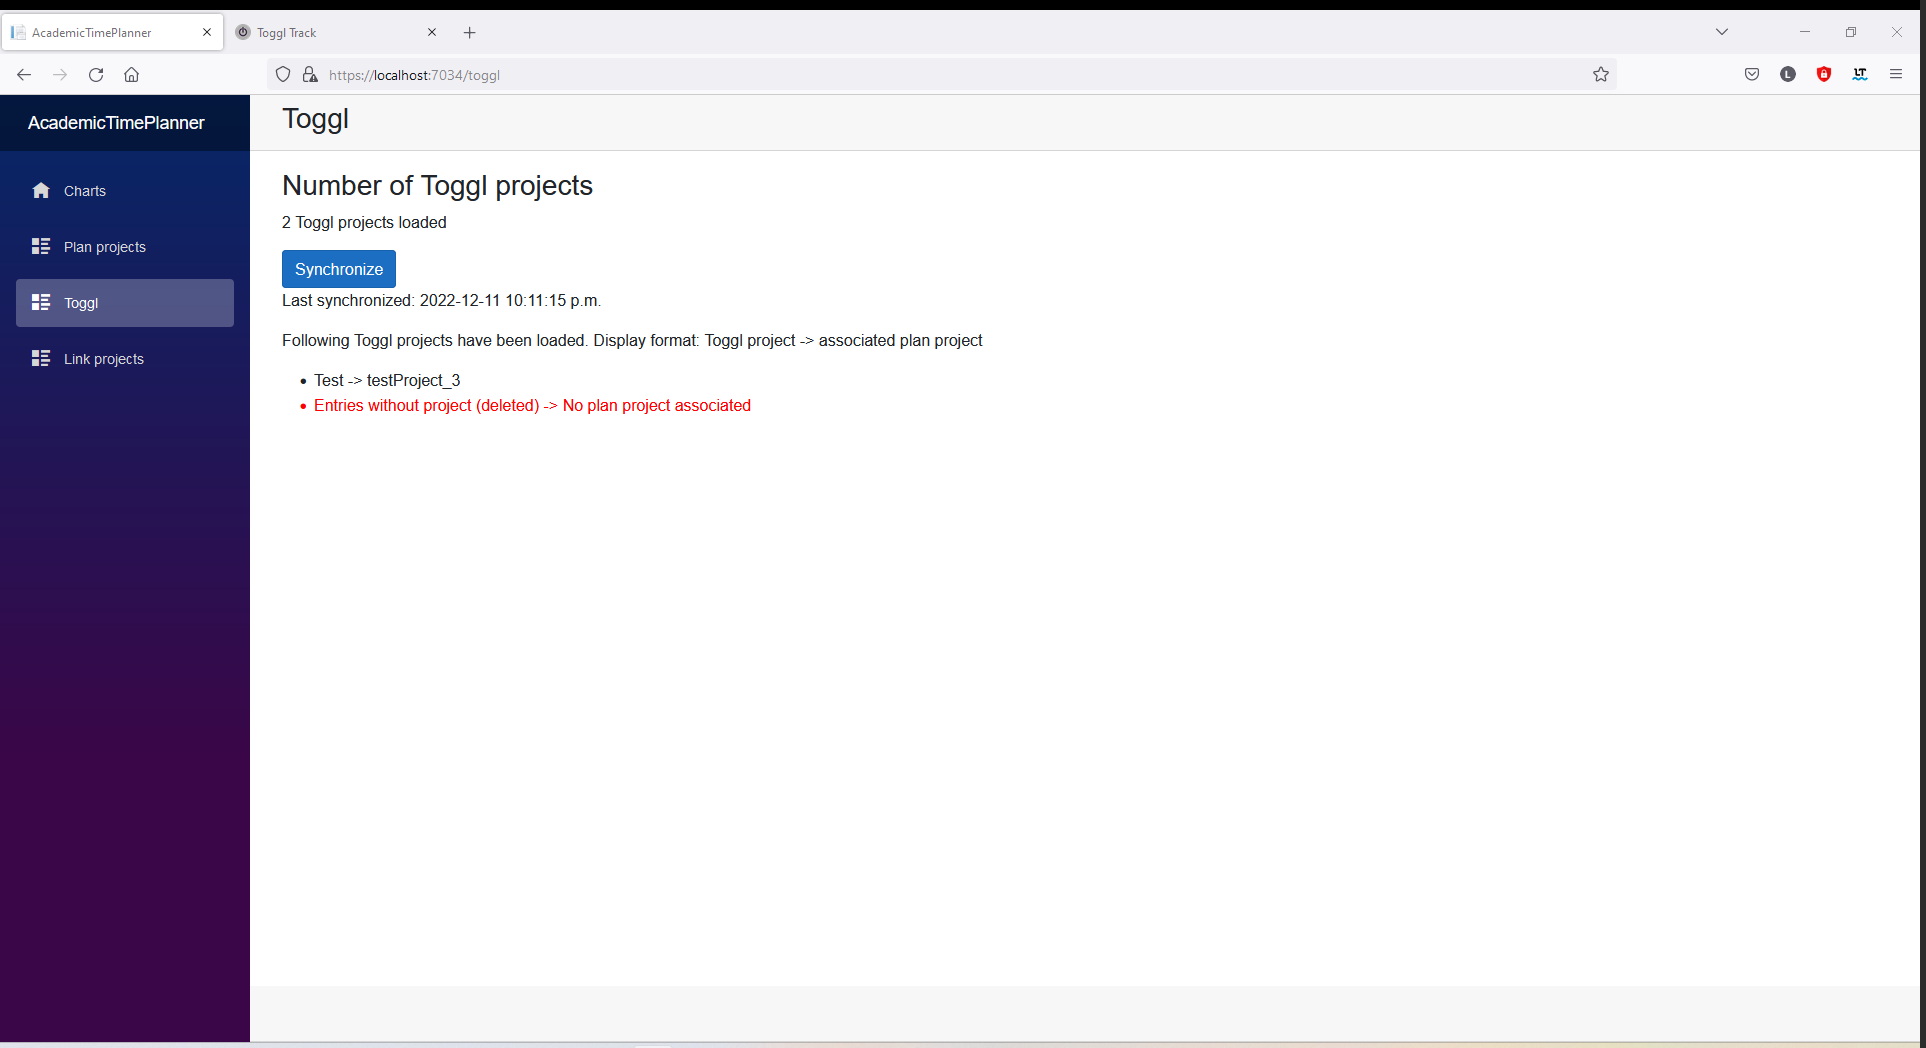
\includegraphics[scale=0.75]{Toggl_deleted}
	\caption{Toggl page after loading of one Toggl project with one deleted project}
	\label{Toggl deleted}
\end{figure}

\section{Front-end of Import, export and creation of plan projects}
The following subsections describe the front-end for import, export and creation of a plan project.

\subsection{Import front-end}
 To import a project the user has to click on the "Browse..." button (see \ref{importButton}). Doing so opens a window where the user can select the projects to be loaded (see \ref{importWindow}). If a project already exists in the ATP, it will be overwritten with the new data, otherwise the plan project is added to the ATP. All loaded plan projects are displayed in a list (see \ref{loadedPlanProjects}).
\begin{figure}[H]
	\centering
	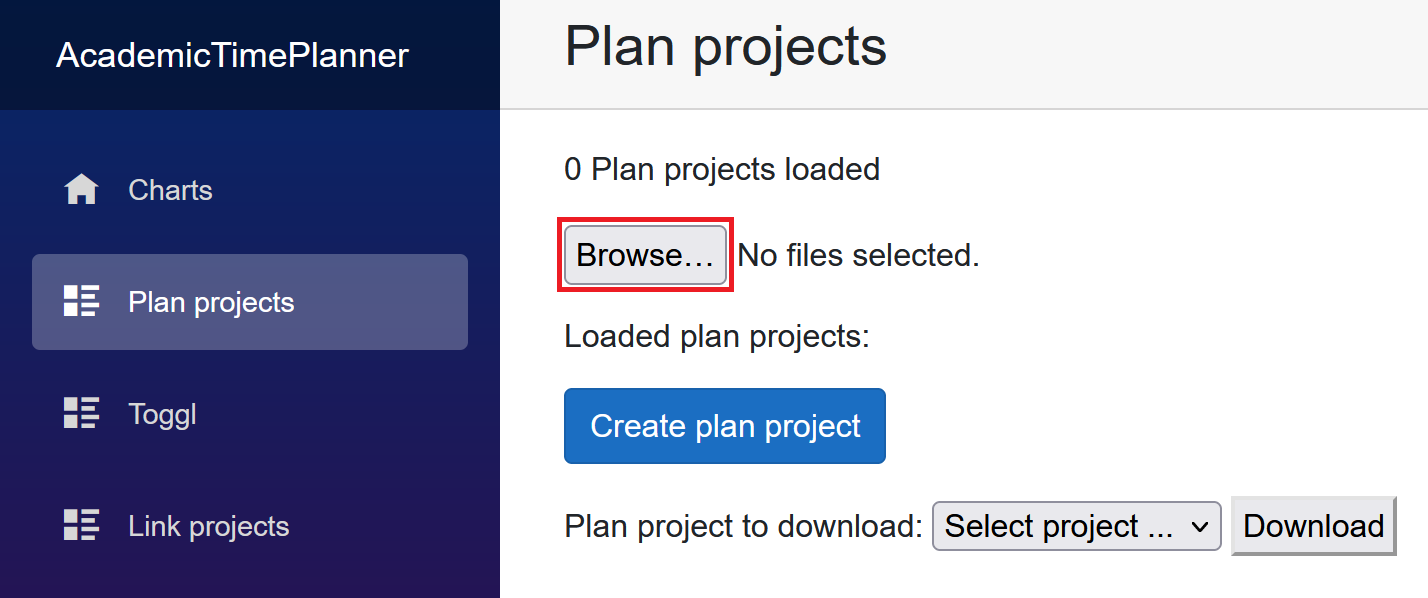
\includegraphics[scale=0.5]{ImportButton}
	\caption{Button to brows files for import}
	\label{importButton}
\end{figure}
\begin{figure}[H]
	\centering
	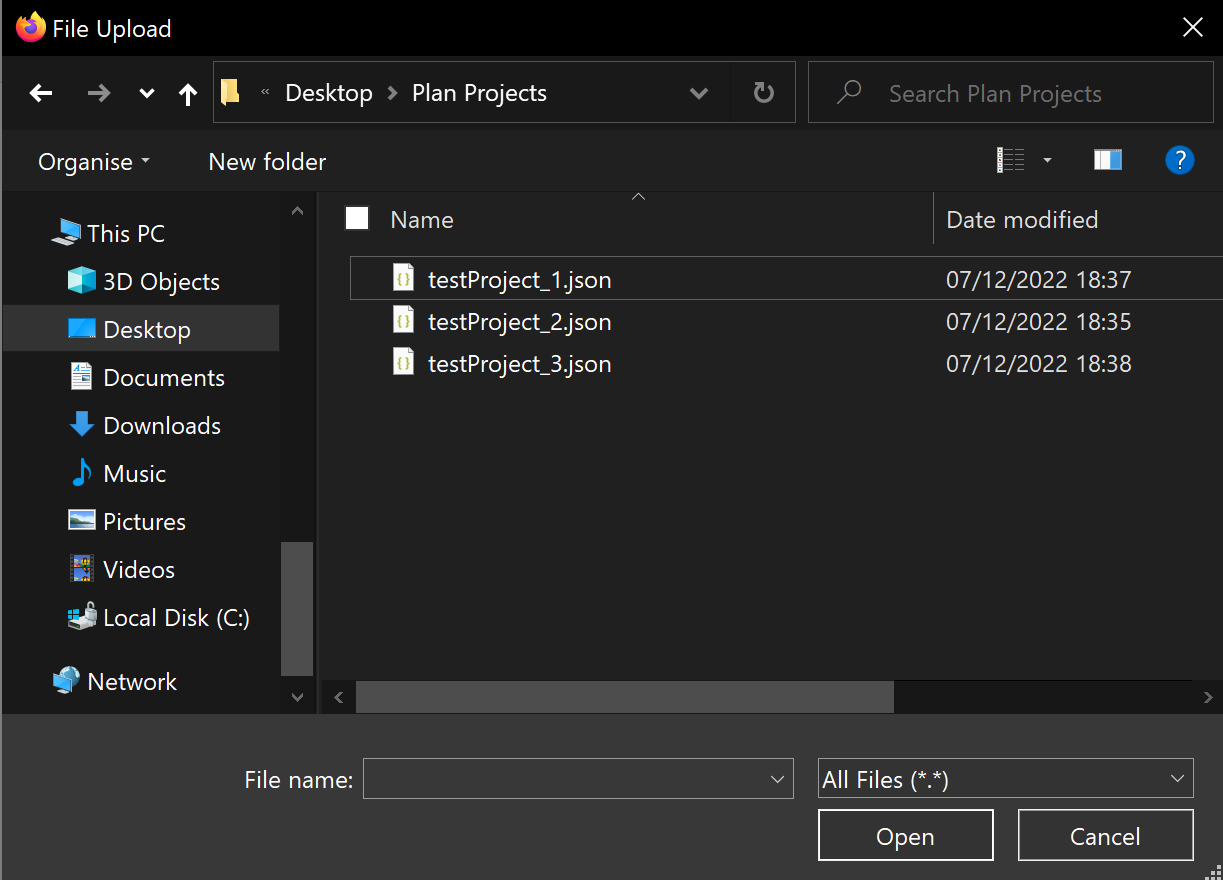
\includegraphics[width=0.6\columnwidth]{ImportProjectWindow}
	\caption{Window to select files for import}
	\label{importWindow}
\end{figure}
\begin{figure}[H]
	\centering
	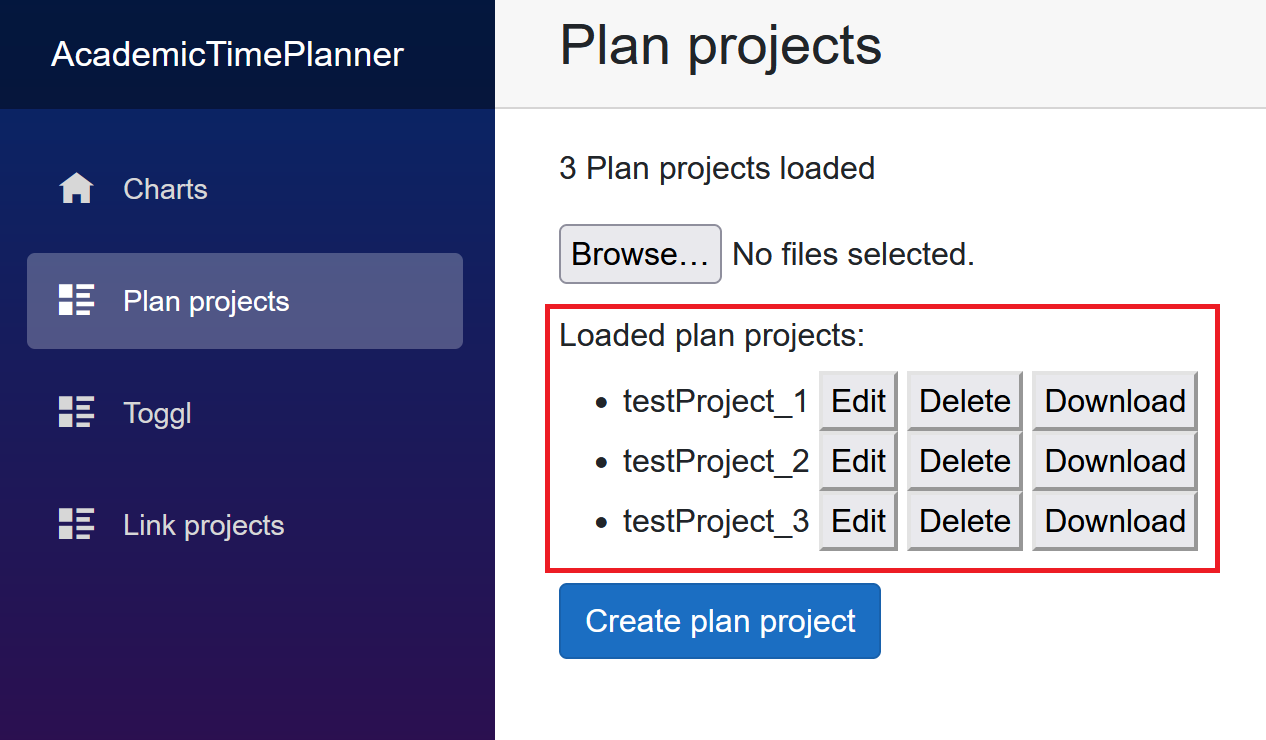
\includegraphics[scale=0.5]{LoadedPlanProjectsList}
	\caption{List of loaded plan projects}
	\label{loadedPlanProjects}
\end{figure}

\subsection{Export front-end}
To export a plan project the user has to select a project with the drop-down menu and then click on the "Download" button next to it (\ref{downloadSelectFile}). This will open the browsers download options like "Save as..." or "Open with...".
\begin{figure}[H]
	\centering
	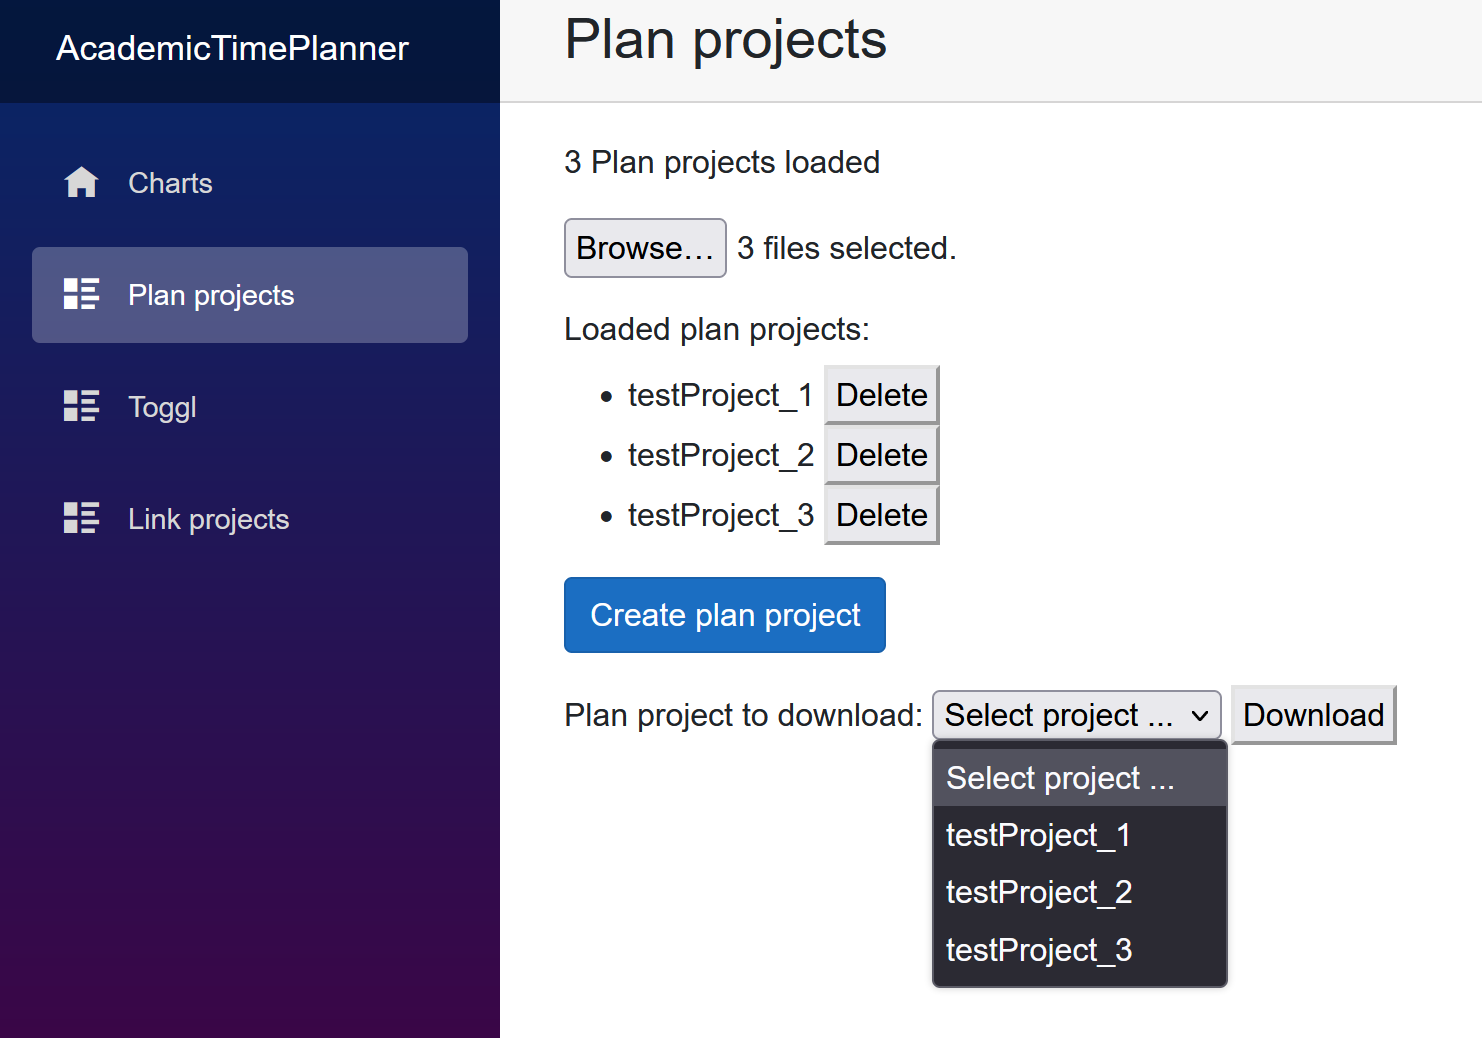
\includegraphics[width=0.6\columnwidth]{DownloadSelectFile}
	\caption{Drop-down to select file and download button}
	\label{downloadSelectFile}
\end{figure}

\subsection{Create plan project front-end}
To create a plan project the user has to click on the "Create plan project" button (see \ref{createPlanProjectButton}). 
\begin{figure}[H]
	\centering
	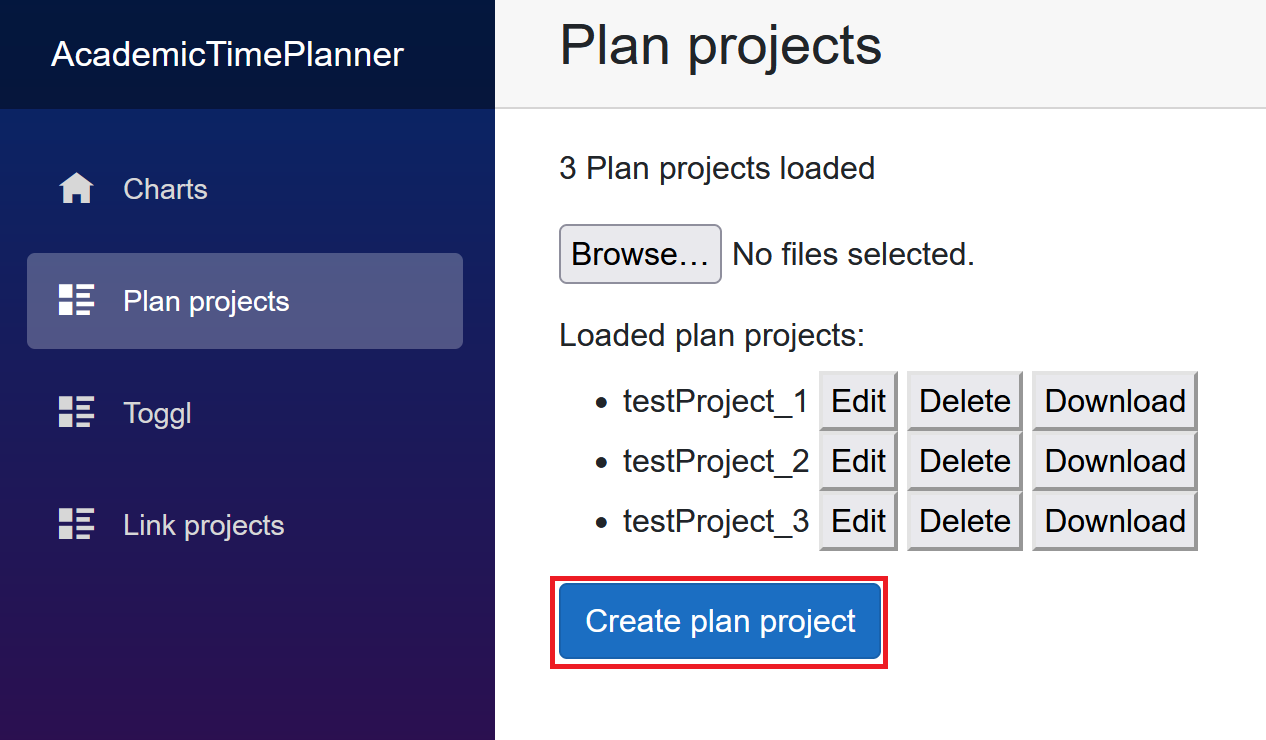
\includegraphics[scale=0.5]{CreatePlanProjectButton}
	\caption{Button to start creating a plan project}
	\label{createPlanProjectButton}
\end{figure}

\subsubsection{Create plan project and plan task}
In the following page the user has to enter the name of the plan project (see \ref{createPlanProject}). Not doing so will result in an error on the final overview page before finalizing the project(see \ref{createFinalOverviewError}). The next page allows the user to create plan tasks by entering a name and clicking on the "Create task" button (see \ref{createPlanTask}). A user can create multiple tasks if desired. This step is optional and the tasks are not needed for the project to function.

\begin{figure}[H]
	\centering
	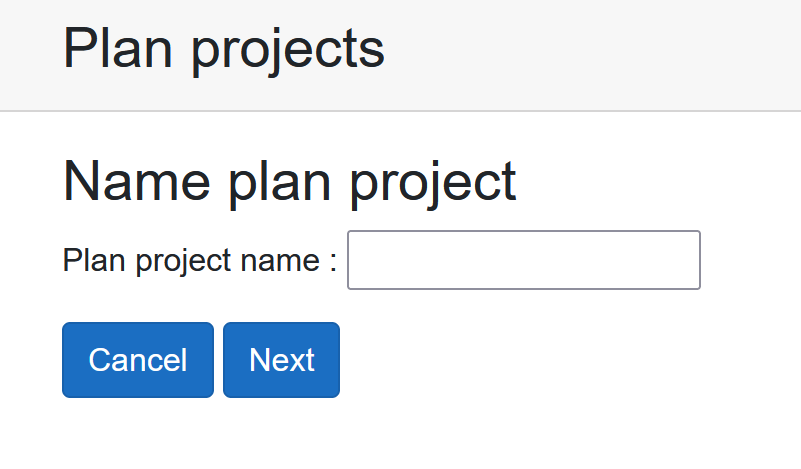
\includegraphics[scale=0.5]{CreatePlanProject}
	\caption{Naming of the plan project}
	\label{createPlanProject}
\end{figure}
\begin{figure}[H]
	\centering
	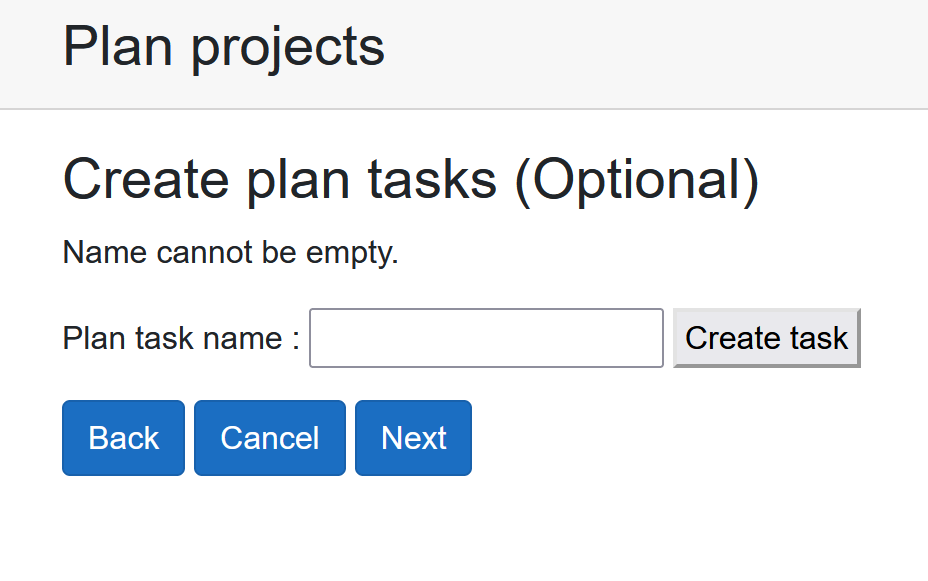
\includegraphics[scale=0.5]{CreatePlanTask}
	\caption{Creating plan tasks}
	\label{createPlanTask}
\end{figure}

\subsubsection{Plan Entries and Plan Entry Repetitions}
On this page the user can choose to create a single plan entry or a plan entry repetition (see \ref{createRepetitionOrEntry}). It is possible to create multiple of both and they can be mixed.
\begin{figure}[H]
	\centering
	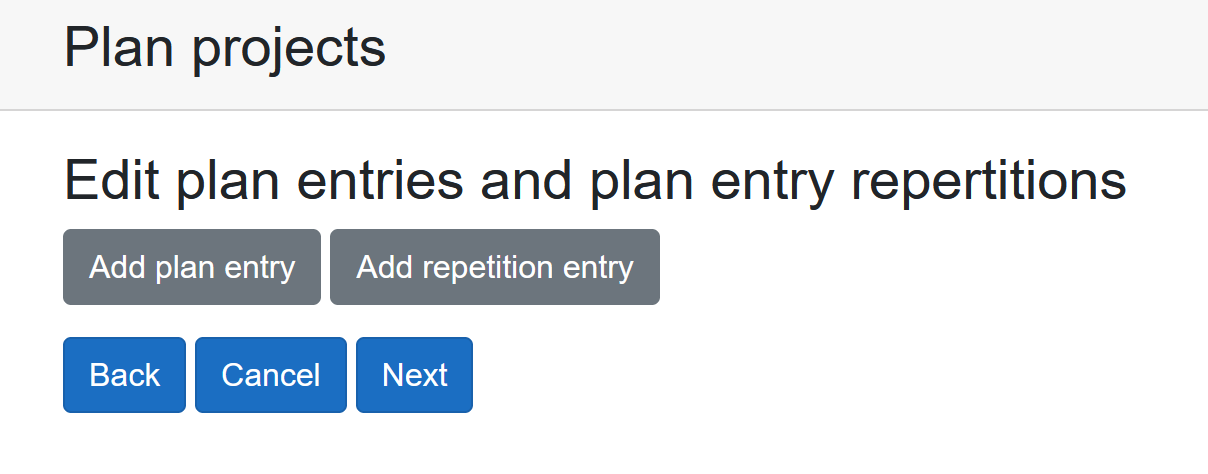
\includegraphics[scale=0.5]{CreateRepetitionOrEntry}
	\caption{Choosing if a single plan entry or a repetition entry should be created}
	\label{createRepetitionOrEntry}
\end{figure}
To create a plan entry all the listed criteria (see \ref{createPlanEntry}) have to be met, otherwise the create plan entry button will not create a plan entry. If plan tasks were created earlier, a task can be linked to the entry. This step is optional as well. After creating a plan entry the user can either create another one or click "Next" to save them and go to the previous page to either create repetition entries, go to finalize or to go back and create tasks.
\begin{figure}[H]
	\centering
	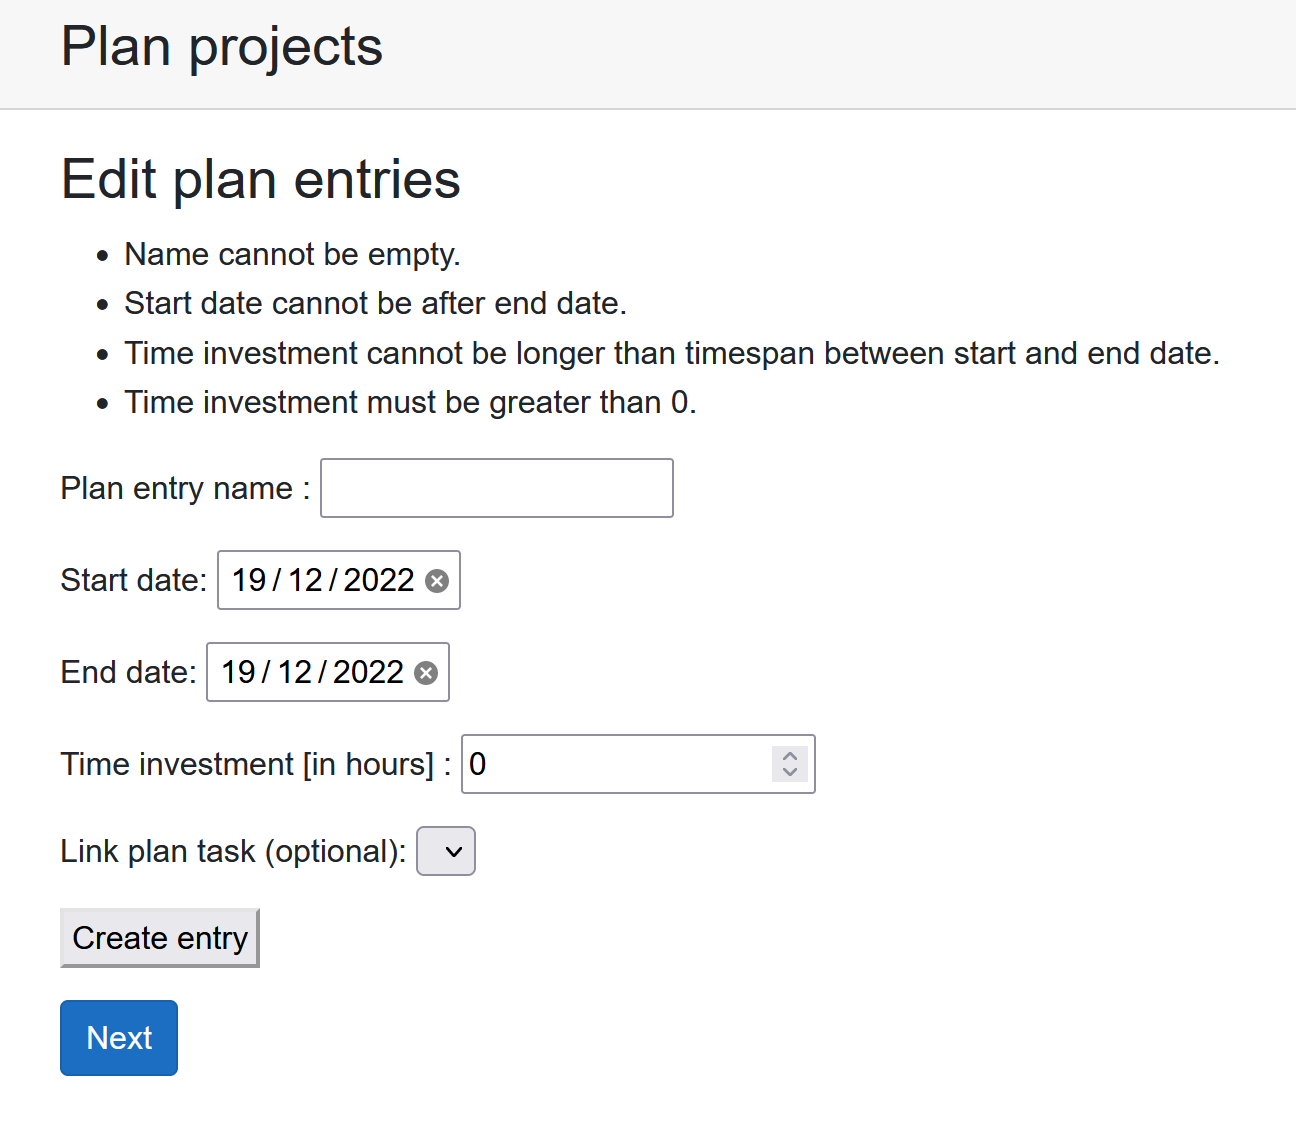
\includegraphics[scale=0.5]{CreatePlanEntry}
	\caption{Creating a plan entry}
	\label{createPlanEntry}
\end{figure}
The creation of a plan entry repetition works similar to the creation of a plan entry. It creates multiple plan entries that repeat after a given interval. By default, the time investment will be distributed evenly over the whole interval. If this is not desired, a time span can be entered which starts at the start of an interval. All criteria are listed for the user to check (see \ref{createRepetitionEntry}).
\begin{figure}[H]
	\centering
	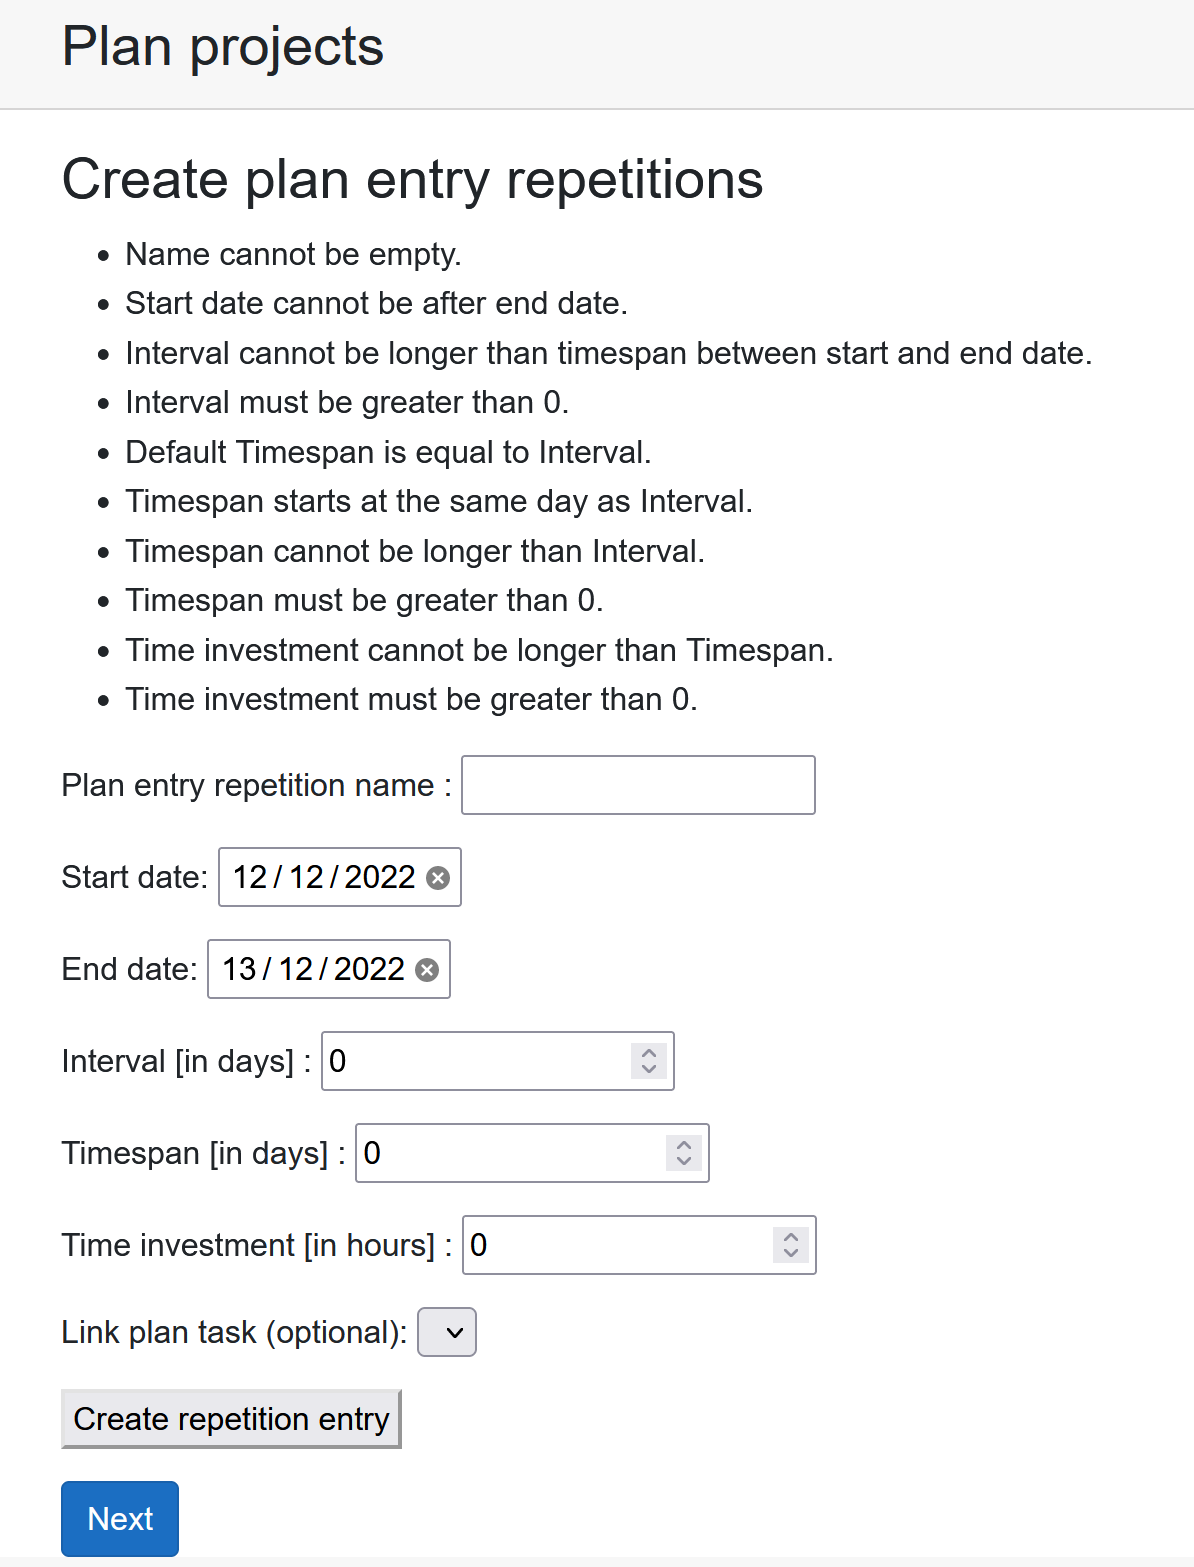
\includegraphics[scale=0.5]{CreateRepetitionEntry}
	\caption{Creating a plan entry repetition}
	\label{createRepetitionEntry}
\end{figure}

\subsubsection{final overview}
In this last page the user can check if all the tasks, plan entries and repetition entries were created (see \ref{createFinalOverview}). If not, the user can go back and create them and in the case of the previous mentioned missing plan project name, the aforementioned error will show (see \ref{createFinalOverviewError}). If everything is in order, the user can click on "Finish" to create the plan project and will be brought back to the initial overview of the projects where the newly created project will be added to the list (see \ref{loadedPlanProjects}).
\begin{figure}[H]
	\centering
	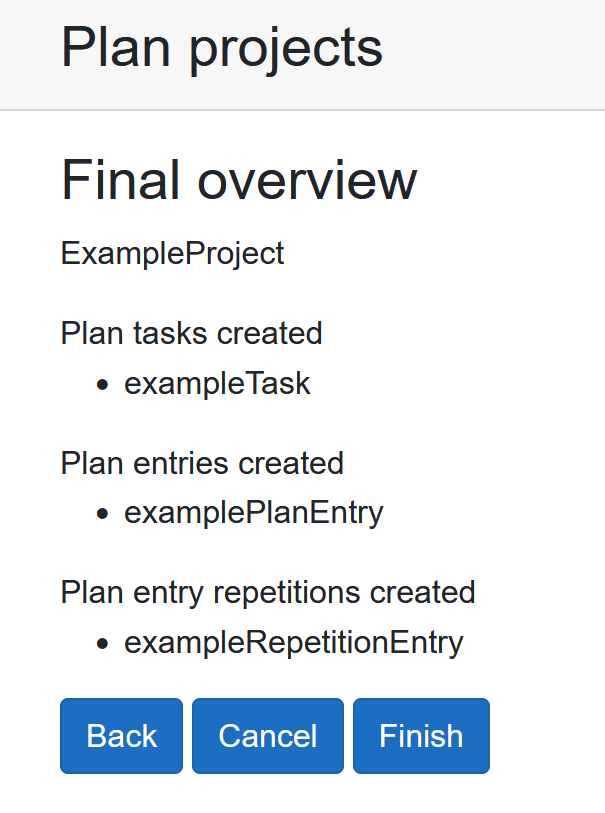
\includegraphics[scale=0.5]{CreateFinalOverview}
	\caption{Final overview of the plan project}
	\label{createFinalOverview}
\end{figure}
\begin{figure}[H]
	\centering
	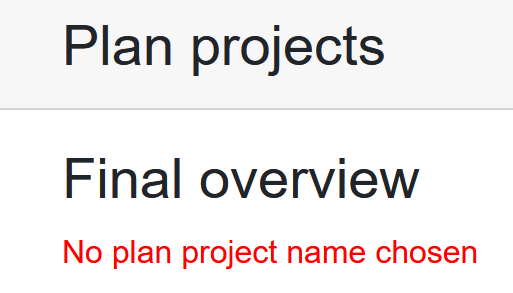
\includegraphics[scale=0.5]{CreateFinalOverviewError}
	\caption{Error message if the plan project was not named}
	\label{createFinalOverviewError}
\end{figure}

\section{Linking of plan projects and Toggl projects} \label{Linking}
The linking page lists the plan projects and the Toggl projects that are present in the ATP as radio buttons. In order to link a Toggl project to a plan projects, users select the two and click on "Link projects". Below the buttons, an overview of the project that have already been linked is displayed (see picture \ref{Linking init}). It is possible to link the same Toggl project to different plan projects. It is also possible to link multiple Toggl projects to one single plan project. To do this, users just have to select the same plan project once again and link it to the Toggl project of their choice (see picture \ref{Linking multiple}).

\begin{figure}[H]
	\centering
	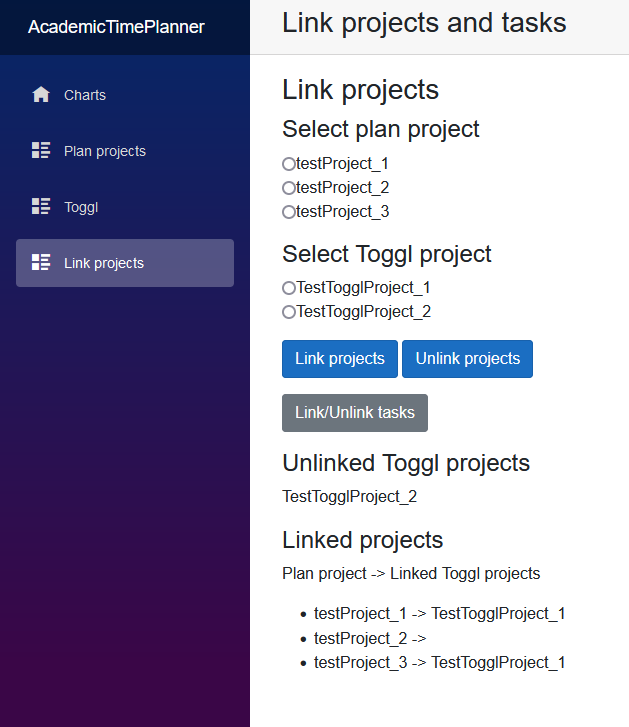
\includegraphics[scale=0.75]{Linking_1}
	\caption{Linking page}
	\label{Linking init}
\end{figure}

\begin{figure}[H]
	\centering
	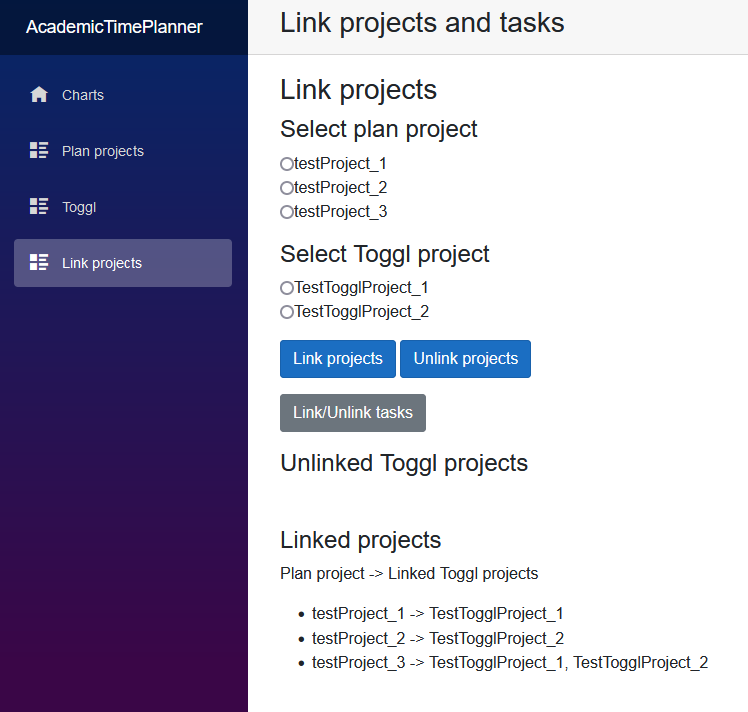
\includegraphics[scale=0.75]{Linking_2}
	\caption{Linking page with multiple Toggl projects linked to one plan project}
	\label{Linking multiple}
\end{figure}

In order to link plan tasks of a plan project to Toggl tasks of the associated Toggl project(s), users may click on "Link tasks", which opens up the according submenu, which looks similar to the project linking menu and works just the same way (see picture \ref{Linking tasks init}). In the overview of the linked tasks, the Toggl project to which a Toggl task belongs is indicated in brackets. Again it is possible to link multiple Toggl tasks to one single plan task (see picture \ref{Linking tasks multiple}), and also to link one Toggl tasks to different plan tasks. By clicking on "Link projects", users may switch back to the project linking menu.

\begin{figure}[H]
	\centering
	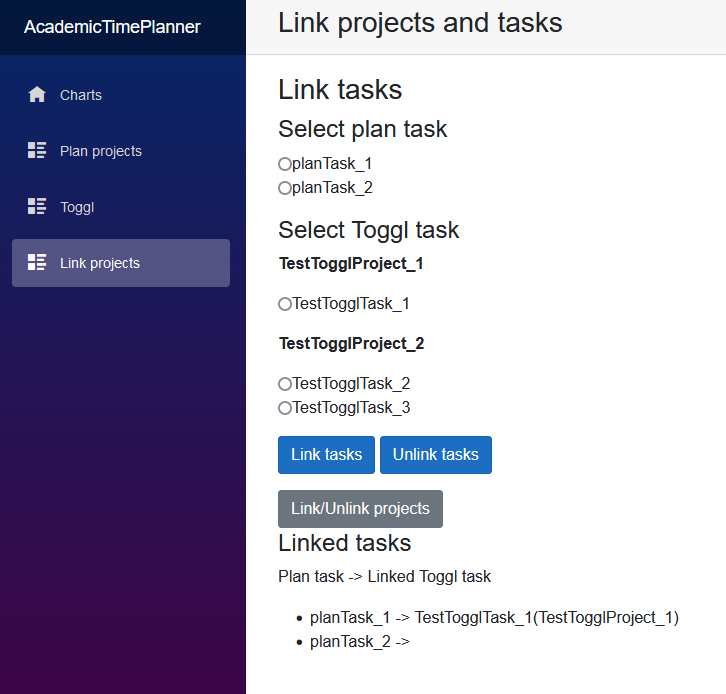
\includegraphics[scale=0.75]{Linking_tasks1}
	\caption{Task linking}
	\label{Linking tasks init}
\end{figure}

\begin{figure}[H]
	\centering
	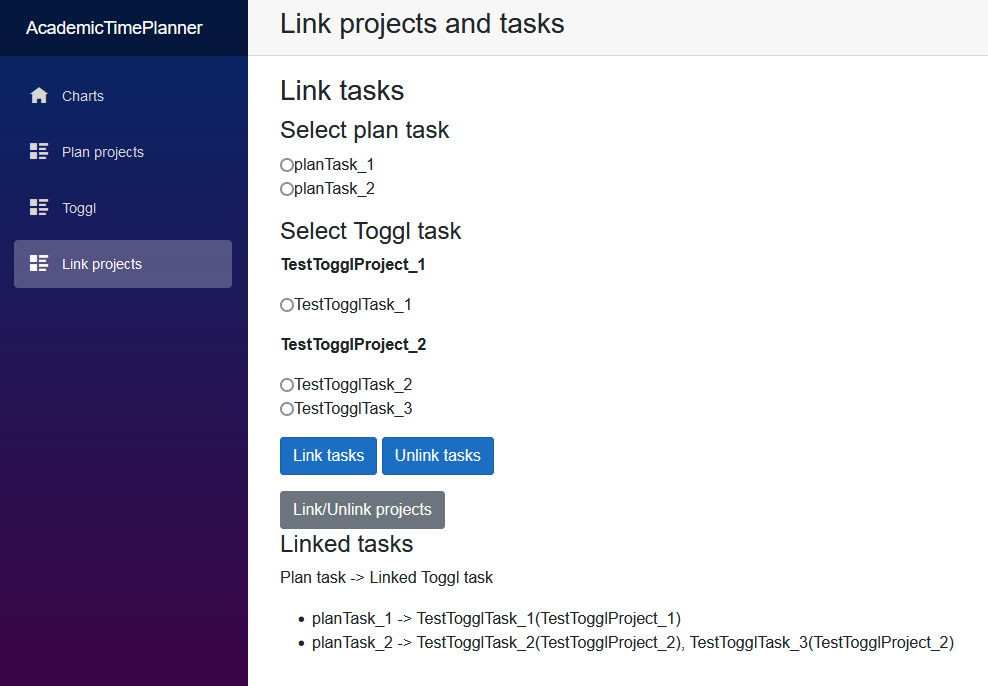
\includegraphics[scale=0.75]{Linking_tasks2}
	\caption{Task linking with multiple Toggl tasks linked to one plan tasks}
	\label{Linking tasks multiple}
\end{figure}